% Graphic for TeX using PGF
% Title: /home/ngoko/Papiers/IPDPS2016/Figures/Search.dia
% Creator: Dia v0.97.3
% CreationDate: Wed Oct  7 12:17:09 2015
% For: ngoko
% \usepackage{tikz}
% The following commands are not supported in PSTricks at present
% We define them conditionally, so when they are implemented,
% this pgf file will use them.
\ifx\du\undefined
  \newlength{\du}
\fi
\setlength{\du}{15\unitlength}
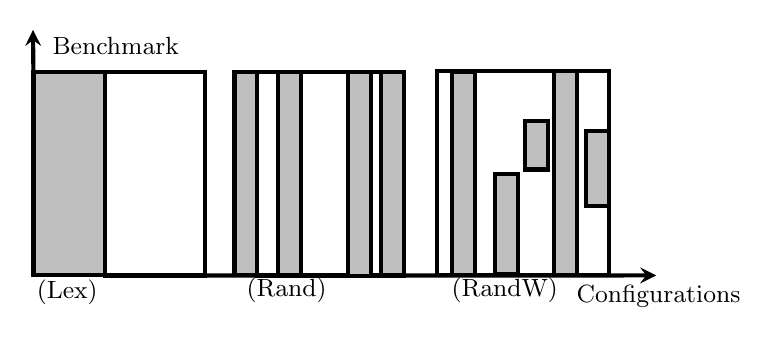
\begin{tikzpicture}
\pgftransformxscale{.5000000}
\pgftransformyscale{-.5000000}
\definecolor{dialinecolor}{rgb}{0.000000, 0.000000, 0.000000}
\pgfsetstrokecolor{dialinecolor}
\definecolor{dialinecolor}{rgb}{1.000000, 1.000000, 1.000000}
\pgfsetfillcolor{dialinecolor}
\definecolor{dialinecolor}{rgb}{0.749020, 0.749020, 0.749020}
\pgfsetfillcolor{dialinecolor}
\fill (15.450000\du,4.950000\du)--(15.450000\du,14.750000\du)--(18.900000\du,14.750000\du)--(18.900000\du,4.950000\du)--cycle;
\pgfsetlinewidth{0.100000\du}
\pgfsetdash{}{0pt}
\pgfsetdash{}{0pt}
\pgfsetmiterjoin
\definecolor{dialinecolor}{rgb}{0.000000, 0.000000, 0.000000}
\pgfsetstrokecolor{dialinecolor}
\draw (15.450000\du,4.950000\du)--(15.450000\du,14.750000\du)--(18.900000\du,14.750000\du)--(18.900000\du,4.950000\du)--cycle;
% setfont left to latex
\definecolor{dialinecolor}{rgb}{0.000000, 0.000000, 0.000000}
\pgfsetstrokecolor{dialinecolor}
\node at (17.175000\du,10.045000\du){};
\definecolor{dialinecolor}{rgb}{1.000000, 1.000000, 1.000000}
\pgfsetfillcolor{dialinecolor}
\fill (18.910000\du,4.955000\du)--(18.910000\du,14.755000\du)--(23.700000\du,14.755000\du)--(23.700000\du,4.955000\du)--cycle;
\pgfsetlinewidth{0.100000\du}
\pgfsetdash{}{0pt}
\pgfsetdash{}{0pt}
\pgfsetmiterjoin
\definecolor{dialinecolor}{rgb}{0.000000, 0.000000, 0.000000}
\pgfsetstrokecolor{dialinecolor}
\draw (18.910000\du,4.955000\du)--(18.910000\du,14.755000\du)--(23.700000\du,14.755000\du)--(23.700000\du,4.955000\du)--cycle;
% setfont left to latex
\definecolor{dialinecolor}{rgb}{0.000000, 0.000000, 0.000000}
\pgfsetstrokecolor{dialinecolor}
\node at (21.305000\du,10.050000\du){};
\pgfsetlinewidth{0.100000\du}
\pgfsetdash{}{0pt}
\pgfsetdash{}{0pt}
\pgfsetbuttcap
{
\definecolor{dialinecolor}{rgb}{0.000000, 0.000000, 0.000000}
\pgfsetfillcolor{dialinecolor}
% was here!!!
\pgfsetarrowsend{stealth}
\definecolor{dialinecolor}{rgb}{0.000000, 0.000000, 0.000000}
\pgfsetstrokecolor{dialinecolor}
\draw (15.450000\du,5.275000\du)--(15.426300\du,2.925000\du);
}
\definecolor{dialinecolor}{rgb}{0.749020, 0.749020, 0.749020}
\pgfsetfillcolor{dialinecolor}
\fill (25.135000\du,4.950000\du)--(25.135000\du,14.750000\du)--(26.235000\du,14.750000\du)--(26.235000\du,4.950000\du)--cycle;
\pgfsetlinewidth{0.100000\du}
\pgfsetdash{}{0pt}
\pgfsetdash{}{0pt}
\pgfsetmiterjoin
\definecolor{dialinecolor}{rgb}{0.000000, 0.000000, 0.000000}
\pgfsetstrokecolor{dialinecolor}
\draw (25.135000\du,4.950000\du)--(25.135000\du,14.750000\du)--(26.235000\du,14.750000\du)--(26.235000\du,4.950000\du)--cycle;
% setfont left to latex
\definecolor{dialinecolor}{rgb}{0.000000, 0.000000, 0.000000}
\pgfsetstrokecolor{dialinecolor}
\node at (25.685000\du,10.045000\du){};
\definecolor{dialinecolor}{rgb}{1.000000, 1.000000, 1.000000}
\pgfsetfillcolor{dialinecolor}
\fill (26.225000\du,4.955000\du)--(26.225000\du,14.755000\du)--(33.225000\du,14.755000\du)--(33.225000\du,4.955000\du)--cycle;
\pgfsetlinewidth{0.100000\du}
\pgfsetdash{}{0pt}
\pgfsetdash{}{0pt}
\pgfsetmiterjoin
\definecolor{dialinecolor}{rgb}{0.000000, 0.000000, 0.000000}
\pgfsetstrokecolor{dialinecolor}
\draw (26.225000\du,4.955000\du)--(26.225000\du,14.755000\du)--(33.225000\du,14.755000\du)--(33.225000\du,4.955000\du)--cycle;
% setfont left to latex
\definecolor{dialinecolor}{rgb}{0.000000, 0.000000, 0.000000}
\pgfsetstrokecolor{dialinecolor}
\node at (29.725000\du,10.050000\du){};
\pgfsetlinewidth{0.100000\du}
\pgfsetdash{}{0pt}
\pgfsetdash{}{0pt}
\pgfsetbuttcap
{
\definecolor{dialinecolor}{rgb}{0.000000, 0.000000, 0.000000}
\pgfsetfillcolor{dialinecolor}
% was here!!!
\pgfsetarrowsend{stealth}
\definecolor{dialinecolor}{rgb}{0.000000, 0.000000, 0.000000}
\pgfsetstrokecolor{dialinecolor}
\draw (23.700000\du,14.755000\du)--(45.451300\du,14.750000\du);
}
\definecolor{dialinecolor}{rgb}{0.749020, 0.749020, 0.749020}
\pgfsetfillcolor{dialinecolor}
\fill (27.235000\du,4.955000\du)--(27.235000\du,14.755000\du)--(28.335000\du,14.755000\du)--(28.335000\du,4.955000\du)--cycle;
\pgfsetlinewidth{0.100000\du}
\pgfsetdash{}{0pt}
\pgfsetdash{}{0pt}
\pgfsetmiterjoin
\definecolor{dialinecolor}{rgb}{0.000000, 0.000000, 0.000000}
\pgfsetstrokecolor{dialinecolor}
\draw (27.235000\du,4.955000\du)--(27.235000\du,14.755000\du)--(28.335000\du,14.755000\du)--(28.335000\du,4.955000\du)--cycle;
% setfont left to latex
\definecolor{dialinecolor}{rgb}{0.000000, 0.000000, 0.000000}
\pgfsetstrokecolor{dialinecolor}
\node at (27.785000\du,10.050000\du){};
\definecolor{dialinecolor}{rgb}{0.749020, 0.749020, 0.749020}
\pgfsetfillcolor{dialinecolor}
\fill (32.185000\du,4.955000\du)--(32.185000\du,14.755000\du)--(33.285000\du,14.755000\du)--(33.285000\du,4.955000\du)--cycle;
\pgfsetlinewidth{0.100000\du}
\pgfsetdash{}{0pt}
\pgfsetdash{}{0pt}
\pgfsetmiterjoin
\definecolor{dialinecolor}{rgb}{0.000000, 0.000000, 0.000000}
\pgfsetstrokecolor{dialinecolor}
\draw (32.185000\du,4.955000\du)--(32.185000\du,14.755000\du)--(33.285000\du,14.755000\du)--(33.285000\du,4.955000\du)--cycle;
% setfont left to latex
\definecolor{dialinecolor}{rgb}{0.000000, 0.000000, 0.000000}
\pgfsetstrokecolor{dialinecolor}
\node at (32.735000\du,10.050000\du){};
\definecolor{dialinecolor}{rgb}{0.749020, 0.749020, 0.749020}
\pgfsetfillcolor{dialinecolor}
\fill (30.595000\du,4.960000\du)--(30.595000\du,14.760000\du)--(31.695000\du,14.760000\du)--(31.695000\du,4.960000\du)--cycle;
\pgfsetlinewidth{0.100000\du}
\pgfsetdash{}{0pt}
\pgfsetdash{}{0pt}
\pgfsetmiterjoin
\definecolor{dialinecolor}{rgb}{0.000000, 0.000000, 0.000000}
\pgfsetstrokecolor{dialinecolor}
\draw (30.595000\du,4.960000\du)--(30.595000\du,14.760000\du)--(31.695000\du,14.760000\du)--(31.695000\du,4.960000\du)--cycle;
% setfont left to latex
\definecolor{dialinecolor}{rgb}{0.000000, 0.000000, 0.000000}
\pgfsetstrokecolor{dialinecolor}
\node at (31.145000\du,10.055000\du){};
\definecolor{dialinecolor}{rgb}{1.000000, 1.000000, 1.000000}
\pgfsetfillcolor{dialinecolor}
\fill (34.876300\du,4.915000\du)--(34.876300\du,14.715000\du)--(43.196300\du,14.715000\du)--(43.196300\du,4.915000\du)--cycle;
\pgfsetlinewidth{0.100000\du}
\pgfsetdash{}{0pt}
\pgfsetdash{}{0pt}
\pgfsetmiterjoin
\definecolor{dialinecolor}{rgb}{0.000000, 0.000000, 0.000000}
\pgfsetstrokecolor{dialinecolor}
\draw (34.876300\du,4.915000\du)--(34.876300\du,14.715000\du)--(43.196300\du,14.715000\du)--(43.196300\du,4.915000\du)--cycle;
% setfont left to latex
\definecolor{dialinecolor}{rgb}{0.000000, 0.000000, 0.000000}
\pgfsetstrokecolor{dialinecolor}
\node at (39.036300\du,10.010000\du){};
% setfont left to latex
\definecolor{dialinecolor}{rgb}{0.000000, 0.000000, 0.000000}
\pgfsetstrokecolor{dialinecolor}
\node[anchor=west] at (20.801300\du,16.225000\du){};
% setfont left to latex
\definecolor{dialinecolor}{rgb}{0.000000, 0.000000, 0.000000}
\pgfsetstrokecolor{dialinecolor}
\node[anchor=west] at (41.076300\du,15.750000\du){\small  Configurations};
% setfont left to latex
\definecolor{dialinecolor}{rgb}{0.000000, 0.000000, 0.000000}
\pgfsetstrokecolor{dialinecolor}
\node[anchor=west] at (15.826300\du,3.675000\du){\small  Benchmark};
% setfont left to latex
\definecolor{dialinecolor}{rgb}{0.000000, 0.000000, 0.000000}
\pgfsetstrokecolor{dialinecolor}
\node[anchor=west] at (15.070700\du,15.550000\du){ \small  (Lex)};
% setfont left to latex
\definecolor{dialinecolor}{rgb}{0.000000, 0.000000, 0.000000}
\pgfsetstrokecolor{dialinecolor}
\node[anchor=west] at (25.175000\du,15.475000\du){\small  (Rand)};
% setfont left to latex
\definecolor{dialinecolor}{rgb}{0.000000, 0.000000, 0.000000}
\pgfsetstrokecolor{dialinecolor}
\node[anchor=west] at (35.050700\du,15.485000\du){\small  (RandW)};
% setfont left to latex
\definecolor{dialinecolor}{rgb}{0.000000, 0.000000, 0.000000}
\pgfsetstrokecolor{dialinecolor}
\node[anchor=west] at (18.800000\du,15.100000\du){};
\definecolor{dialinecolor}{rgb}{0.749020, 0.749020, 0.749020}
\pgfsetfillcolor{dialinecolor}
\fill (35.610000\du,4.930000\du)--(35.610000\du,14.730000\du)--(36.710000\du,14.730000\du)--(36.710000\du,4.930000\du)--cycle;
\pgfsetlinewidth{0.100000\du}
\pgfsetdash{}{0pt}
\pgfsetdash{}{0pt}
\pgfsetmiterjoin
\definecolor{dialinecolor}{rgb}{0.000000, 0.000000, 0.000000}
\pgfsetstrokecolor{dialinecolor}
\draw (35.610000\du,4.930000\du)--(35.610000\du,14.730000\du)--(36.710000\du,14.730000\du)--(36.710000\du,4.930000\du)--cycle;
% setfont left to latex
\definecolor{dialinecolor}{rgb}{0.000000, 0.000000, 0.000000}
\pgfsetstrokecolor{dialinecolor}
\node at (36.160000\du,10.025000\du){};
\definecolor{dialinecolor}{rgb}{0.749020, 0.749020, 0.749020}
\pgfsetfillcolor{dialinecolor}
\fill (40.520000\du,4.910000\du)--(40.520000\du,14.710000\du)--(41.620000\du,14.710000\du)--(41.620000\du,4.910000\du)--cycle;
\pgfsetlinewidth{0.100000\du}
\pgfsetdash{}{0pt}
\pgfsetdash{}{0pt}
\pgfsetmiterjoin
\definecolor{dialinecolor}{rgb}{0.000000, 0.000000, 0.000000}
\pgfsetstrokecolor{dialinecolor}
\draw (40.520000\du,4.910000\du)--(40.520000\du,14.710000\du)--(41.620000\du,14.710000\du)--(41.620000\du,4.910000\du)--cycle;
% setfont left to latex
\definecolor{dialinecolor}{rgb}{0.000000, 0.000000, 0.000000}
\pgfsetstrokecolor{dialinecolor}
\node at (41.070000\du,10.005000\du){};
\definecolor{dialinecolor}{rgb}{0.749020, 0.749020, 0.749020}
\pgfsetfillcolor{dialinecolor}
\fill (37.680000\du,9.850000\du)--(37.680000\du,14.700000\du)--(38.780000\du,14.700000\du)--(38.780000\du,9.850000\du)--cycle;
\pgfsetlinewidth{0.100000\du}
\pgfsetdash{}{0pt}
\pgfsetdash{}{0pt}
\pgfsetmiterjoin
\definecolor{dialinecolor}{rgb}{0.000000, 0.000000, 0.000000}
\pgfsetstrokecolor{dialinecolor}
\draw (37.680000\du,9.850000\du)--(37.680000\du,14.700000\du)--(38.780000\du,14.700000\du)--(38.780000\du,9.850000\du)--cycle;
% setfont left to latex
\definecolor{dialinecolor}{rgb}{0.000000, 0.000000, 0.000000}
\pgfsetstrokecolor{dialinecolor}
\node at (38.230000\du,12.470000\du){};
\definecolor{dialinecolor}{rgb}{0.749020, 0.749020, 0.749020}
\pgfsetfillcolor{dialinecolor}
\fill (42.090000\du,7.800000\du)--(42.090000\du,11.400000\du)--(43.190000\du,11.400000\du)--(43.190000\du,7.800000\du)--cycle;
\pgfsetlinewidth{0.100000\du}
\pgfsetdash{}{0pt}
\pgfsetdash{}{0pt}
\pgfsetmiterjoin
\definecolor{dialinecolor}{rgb}{0.000000, 0.000000, 0.000000}
\pgfsetstrokecolor{dialinecolor}
\draw (42.090000\du,7.800000\du)--(42.090000\du,11.400000\du)--(43.190000\du,11.400000\du)--(43.190000\du,7.800000\du)--cycle;
% setfont left to latex
\definecolor{dialinecolor}{rgb}{0.000000, 0.000000, 0.000000}
\pgfsetstrokecolor{dialinecolor}
\node at (42.640000\du,9.795000\du){};
\definecolor{dialinecolor}{rgb}{0.749020, 0.749020, 0.749020}
\pgfsetfillcolor{dialinecolor}
\fill (39.150000\du,7.300000\du)--(39.150000\du,9.650000\du)--(40.250000\du,9.650000\du)--(40.250000\du,7.300000\du)--cycle;
\pgfsetlinewidth{0.100000\du}
\pgfsetdash{}{0pt}
\pgfsetdash{}{0pt}
\pgfsetmiterjoin
\definecolor{dialinecolor}{rgb}{0.000000, 0.000000, 0.000000}
\pgfsetstrokecolor{dialinecolor}
\draw (39.150000\du,7.300000\du)--(39.150000\du,9.650000\du)--(40.250000\du,9.650000\du)--(40.250000\du,7.300000\du)--cycle;
% setfont left to latex
\definecolor{dialinecolor}{rgb}{0.000000, 0.000000, 0.000000}
\pgfsetstrokecolor{dialinecolor}
\node at (39.700000\du,8.670000\du){};
\end{tikzpicture}
